% Some commands used in this file
%\newcommand{\package}{\emph}

\chapter{Conclusion \& Future Work}
\label{chap:conclusion}
During the project, the necessary maintenance is made for ITU-AGVs, new embedded software is developed and it is designed to be ready for communication with ROS. A ROS package is created for ITU-AGVs which contain all the source codes, scripts, launch files, urdf files and custom messages. A 3D model is built for use in visual simulations and representation, the created model is implemented in ROS environment. It is possible in the future to use this model for simulation of navigation, SLAM, multi-robot system and various trials that would be subject of other theses, works or learning projects at ITU Robotics Laboratory. 
\par
ITU-AGVs are equipped with numerous sensors, and all the sensors are ready to be used, their sensor packages are installed and tested, launch files for different sensor combinations are created. 
\par
Teleoperation application is developed and tested. ITU-AGVs can simply be moved using a joystick. This would help to transport the robots to the desired application areas as well as data collecting. Thesis students who only focuses on certain data processing on a moving robot, i.e. RGBD or laser data, does not need to deal with the background process. They can directly do the teleoperation. 
\par
The vital step of acquiring odometry information is done. This information is directly provided for future studies that strictly depend on it. 
Lastly an offline map is built by recording selected data and combining them. This is the first part into mapping and it should be continued to autonomously online mapping. 
\par
The necessary basis is formed as desired with both embedded and computer software. This solved the problem of ITU-AGVs for being out-of-date and made a contribution to ITU Robotics Laboratory. 
\par
Based upon this work, many improvements can be initiated in the future. The created ROS package is a prototype since the process of learning proceeded in parallel with the project. The package can be separated into specific packages, and a metapackage for them can be created. The codes can be review in order to use in newer distributions of ROS. 
	\begin{figure}
		\centering
		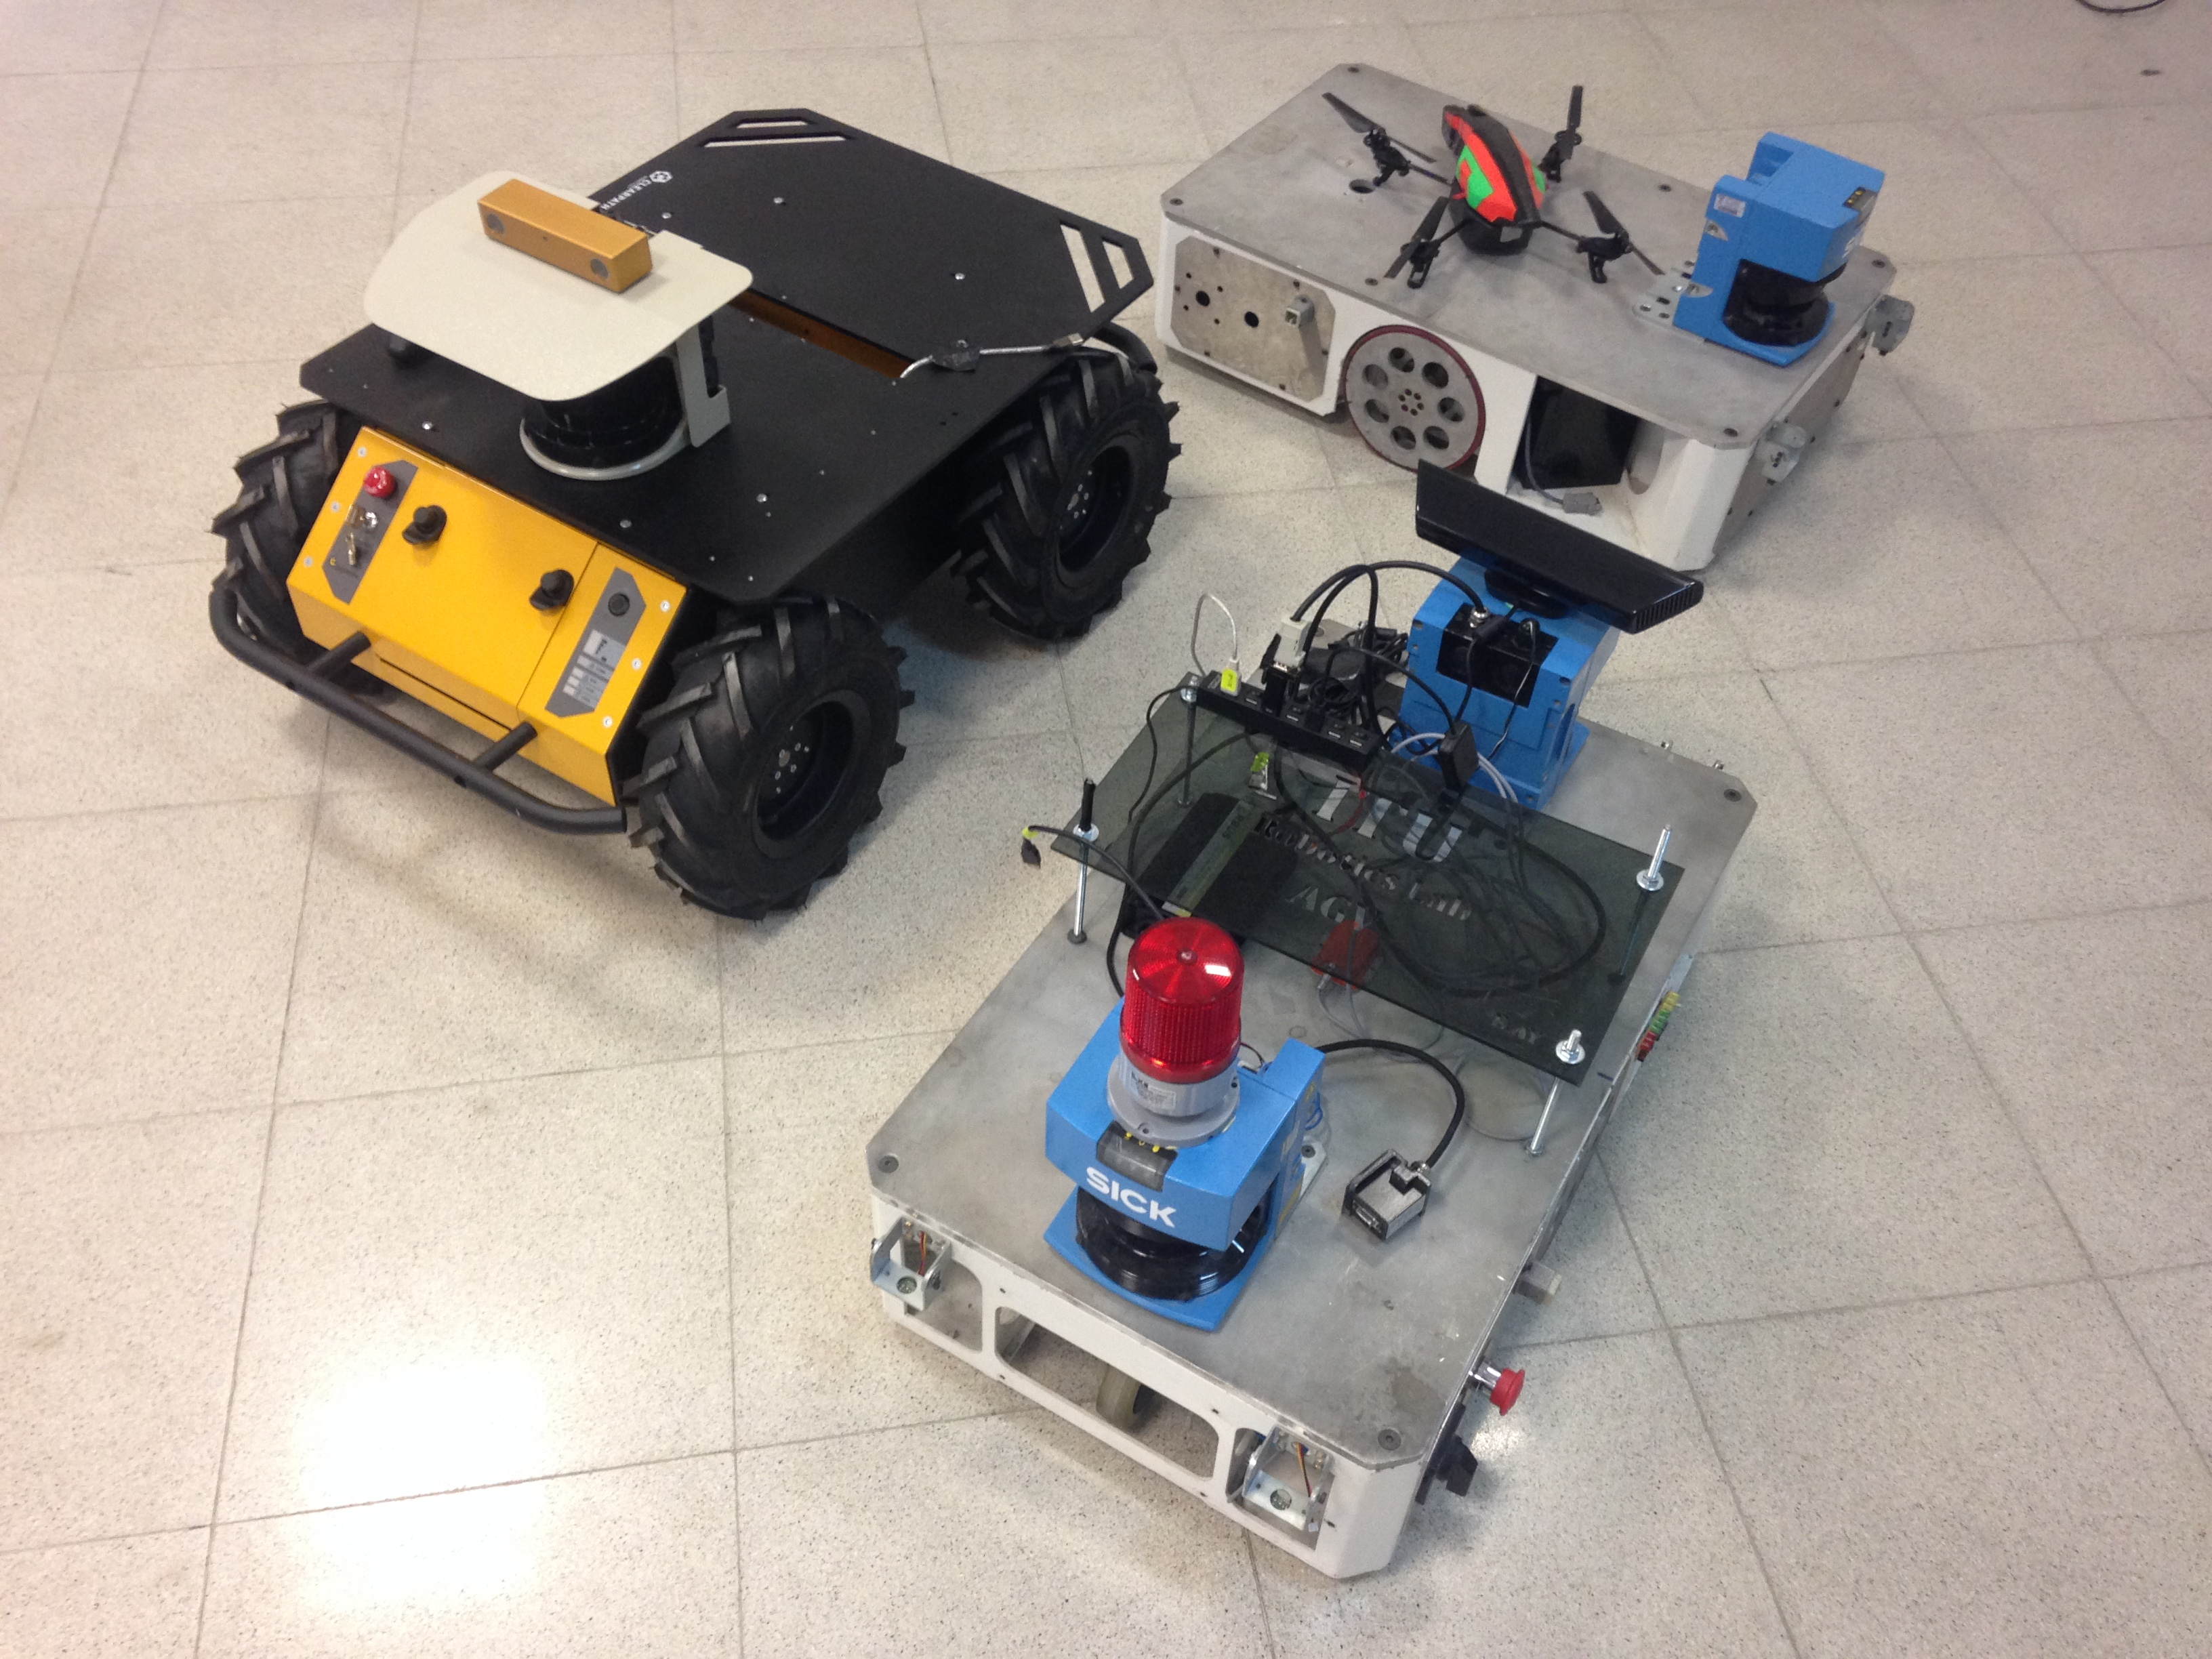
\includegraphics[scale=0.11]{images/husky}
		\caption{Husky robot, ITU-AGVs and AR Drone quadcopter at ITU Robotics Laboratory}
		\label{fig:husky}
	\end{figure}
\par
It is possible to develop autonomous applications based on this package. Navigation, SLAM, loop closure applications or swarm systems can be realized as well as heterogeneous robot groups. In ITU Robotics Laboratory, a group of robots are strategically gathered (Figure ~\ref{fig:husky}). A new outdoor robot kit Husky is bought and it is planned to work on with heterogeneous groups of Husky robot, AR Drone quadcopter and ITU-AGVs in outdoor or indoor, depending on the groups. ROS plays a significant role in the future projects and the package created in this project is the base step for this target. 
